\begin{XeClass}{ChecksumFileSystem}
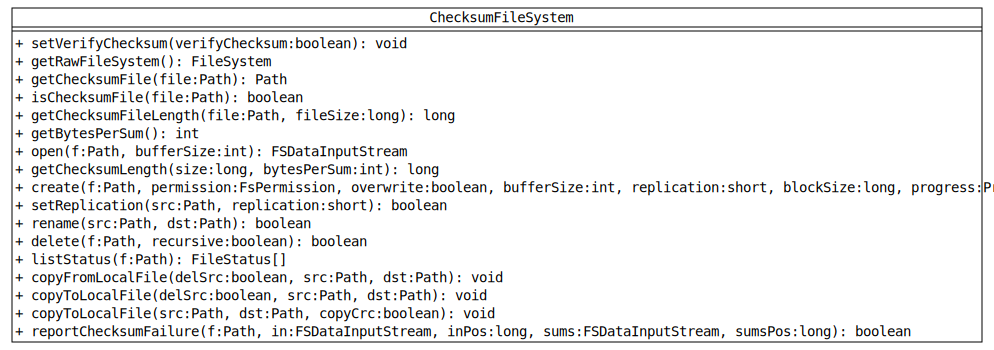
\includegraphics[width=10cm]{cdig/ChecksumFileSystem.png}
     
 ChecksumFileSystem继承自FilterFileSystem
 提供一个基本的文件校验系统的实现,
 通过校验和文件可以检查原生文件系统的完整性,
 冗余备份的情况下,多个节点储存,以防止校验和本身损坏。
 HDFS 会对写入的所有数据计算校验和(checksum),并在读取数据时验证校验和。
 针对指定字节的数目计算校验和。字节数默认是512 字节,可以通过bytesPerChecksum属性设置。
 含义是每512个字节会生成一个4字节长(32位)的CRC检验和。
 Datanode 在保存数据前负责验证checksum。
 client 会把数据和校验和一起发送到一个由多个datanode 组成的队列中,
 最后一个Datanode 负责验证checksum。
 如果验证失败,会抛出一个ChecksumException。客户端需要处理这种异常。   
 客户端从datanode读取数据时,也会验证checksum。
 每个Datanode 都保存了一个验证checksum的日志。
 每次客户端成功验证一个数据块后,都会告知datanode,datanode会更新日志。
 每个datanode 也会在一个后台线程中运行一个DataBlockScanner,
 定期验证这个 datanode 上的所有数据块。   
 在用Hadoop fs get命令读取文件时,可以用-ignoreCrc忽略验证。
 如果是通过FileSystem API 读取时,可以通过setVerifyChecksum(false),忽略验证。 

    \begin{XeMethod}{\XePublic}{void}{setVerifyChecksum}
         
 设置是否检验了校验和

    \end{XeMethod}

    \begin{XeMethod}{\XePublic}{FileSystem}{getRawFileSystem}
         
 获取原生文件系统

    \end{XeMethod}

    \begin{XeMethod}{\XePublic}{Path}{getChecksumFile}
         
 返回检验和文件关联文件的文件名

    \end{XeMethod}

    \begin{XeMethod}{\XePublic}{boolean}{isChecksumFile}
         
 当文件名是校验和文件名时,返回真值

    \end{XeMethod}

    \begin{XeMethod}{\XePublic}{long}{getChecksumFileLength}
         
 返回校验和文件的长度和源文件的大小

    \end{XeMethod}

    \begin{XeMethod}{\XePublic}{int}{getBytesPerSum}
         
 返回每个byte长度的校验和的数据字节数

    \end{XeMethod}

    \begin{XeMethod}{\XePublic}{FSDataInputStream}{open}
         
 在指定的路径下开启一个FSData的输入流

    \end{XeMethod}

    \begin{XeMethod}{\XePublic}{long}{getChecksumLength}
         
 按byte计算校验和文件的长度

    \end{XeMethod}

    \begin{XeMethod}{\XePublic}{FSDataOutputStream}{create}
         
 根据文件路径和权限创建文件输出流

    \end{XeMethod}

    \begin{XeMethod}{\XePublic}{boolean}{setReplication}
         
 Set replication for an existing file.
 为一个已经存在的文件进行复制操作
 Implement the abstract <tt>setReplication</tt> of <tt>FileSystem</tt>
 false if file does not exist or is a directory

    \end{XeMethod}

    \begin{XeMethod}{\XePublic}{boolean}{rename}
         
 重命名 files/dirs

    \end{XeMethod}

    \begin{XeMethod}{\XePublic}{boolean}{delete}
         
 在校验和文件系统中执行删除操作,
 可以选择是否递归删除

    \end{XeMethod}

    \begin{XeMethod}{\XePublic}{FileStatus[]}{listStatus}
         
 如果路径是个目录,列出给出路径下的文件和路径的状态

    \end{XeMethod}

    \begin{XeMethod}{\XePublic}{void}{copyFromLocalFile}
         
 从本地文件系统进行复制

    \end{XeMethod}

    \begin{XeMethod}{\XePublic}{void}{copyToLocalFile}
         
 复制到本地文件系统

    \end{XeMethod}

    \begin{XeMethod}{\XePublic}{void}{copyToLocalFile}
         
 src在文件系统下,dst在本地硬盘上
 从文件系统中复制到本地的dst名
 如果src和dst指向的路径, 参数copyCrc决定是否复制CRC文件

    \end{XeMethod}

    \begin{XeMethod}{\XePublic}{boolean}{reportChecksumFailure}
         
 给文件系统报告一个校验和的错误

    \end{XeMethod}

    \begin{XeInnerClass}{ChecksumFSInputChecker}
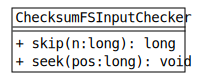
\includegraphics[width=10cm]{cdig/ChecksumFSInputChecker.png}
         
 文件系统的输入流的校验和类
 确认数据和校验和是否匹配

        \begin{XeMethod}{\XePrivate}{long}{getChecksumFilePos}
             
 获取文件的校验和位置

        \end{XeMethod}

        \begin{XeMethod}{\XeProtected}{long}{getChunkPosition}
             
 获取块的校验和位置

        \end{XeMethod}

        \begin{XeMethod}{\XePublic}{int}{read}
             
 检查校验和,读取数据到b字节数组
 返回读取的字节数

        \end{XeMethod}

        \begin{XeMethod}{\XePublic}{void}{close}
             
 关闭数据输入流
 关闭校验和输入流

        \end{XeMethod}

        \begin{XeMethod}{\XePublic}{boolean}{seekToNewSource}
             
 读入指针移动到新的地方

        \end{XeMethod}

        \begin{XeMethod}{\XeProtected}{int}{readChunk}
             
 如果需要校验就进行检验和,
 然后读取文件中的块数据。

        \end{XeMethod}

        \begin{XeMethod}{\XePrivate}{long}{getFileLength}
             
 获取文件的长度

        \end{XeMethod}

        \begin{XeMethod}{\XePublic \\ \XeSync}{long}{skip}
             
 忽略或者弃用输入流中n byte的数据
 在总计忽略或者弃用n byte的数据前,用Skip方法忽略一些小的bytes
 实际忽略的byte数会被返回。如果n是负数,则不忽略任何byte。

        \end{XeMethod}

        \begin{XeMethod}{\XePublic \\ \XeSync}{void}{seek}
             
 在流中查找给定的位置
 下一次read()从此位置开始
 查找的数据块损坏时抛出ChecksumException 

        \end{XeMethod}

    \end{XeInnerClass}
    \begin{XeInnerClass}{ChecksumFSOutputSummer}
\includegraphics[width=10cm]{cdig/ChecksumFSOutputSummer.png}
         
 文件系统的输出流的校验和类
 确认数据和校验和是否匹配

        \begin{XeMethod}{\XePublic}{void}{close}
             
 关闭数据输出流,校验和输出流

        \end{XeMethod}

        \begin{XeMethod}{\XeProtected}{void}{writeChunk}
             
 写入块数据,包括原生数据和校验和

        \end{XeMethod}

    \end{XeInnerClass}
\end{XeClass}
